% implementierung.tex
Dieses Kapitel gibt einen Einblick in den Workflow der R-Paket Erstellung und die Konzepte der Implementierung. Weiters werden wichtige Algorithmen im Pseudocode dargestellt und erläutert. Als Einstiegspunkt für die Implementierung stand eine C-Referenzimplementierung\footnote{\url{http://vashe.org/turbo/turbo_example.c} [01.06.2016]} zur Verfügung, die den Dekodier-Algorithmus für Turbo-Kodes beinhaltet, jedoch für ein konkretes Beispiel. Der Algorithmus musste angepasst und erweitert werden um für allgemeine Faltungskodes verwendbar zu sein.
\\
\\
In Kapitel~\ref{kapitel:implementierung_rpaket} wird der Workflow zur Entwicklung eigener R-Pakete beschrieben. In Kapitel \ref{kapitel:implementierung_faltungskodierer} wird die implementierte Faltungskodierer-Datenstruktur erläutert. Anschließend wird der Kodierungsalgorithmus in Kapitel~\ref{kapitel:implementierung_kodierung} erklärt, gefolgt vom Dekodierungsalgorithmus in Kapitel~\ref{kapitel:implementierung_dekodierung}. Weiters wird die Umsetzung der Funktion zum Verrauschen einer Nachricht in Kapitel~\ref{kapitel:implementierung_noise} präsentiert. Kapitel~\ref{kapitel:implementierung_punktierung} beinhaltet die Implementierung der Punktierung. Schließlich geben die Kapitel~\ref{kapitel:implementierung_simulation} bzw. \ref{kapitel:implementierung_visualisierung} einen Einblick in die Implementierung der Simulation bzw. Visualisierungen.
\\
\\
Bei den Implementierungen der Funktionen ab Kapitel~\ref{kapitel:implementierung_faltungskodierer} werden alle Parameter überprüft, ob die Werte korrekt übergeben wurden. Auf eine Erklärung dieser Überprüfungen wird, außer bei Funktionen, die andernfalls unvollständig beschrieben wären, verzichtet. Darüber hinaus sind für den Großteil der Parameter Standardwerte hinterlegt. Diese Standardwerte werden bei der Ausführung der Funktion verwendet, sollte ein Parameter vom Benutzer nicht übergeben worden sein.
\section{R-Paket Entwicklung}
\label{kapitel:implementierung_rpaket}
Dieses Kapitel setzt die Installation der R-Pakete \texttt{roxygen2} und \texttt{devtools} (siehe Kapitel~\ref{kapitel:R}) voraus. Zur Installation eines Pakets kann im RStudio im \emph{Packages}-Tab die \emph{Install}-Funktion oder der Befehl in Zeile~1 des Listings~\ref{lst:install} verwendet werden.
\\
\begin{lstlisting}[caption=Installation eines R-Pakets und dessen Abhängigkeiten, label={lst:install}, float=!th]
install.package(<package-name>)
devtools::install_deps(pkg = <package-name>, dependencies = TRUE)
\end{lstlisting}
Bei der Verwendung von C/C++-Code werden ein entsprechender Compiler sowie, abhängig vom Betriebssystem, weitere Tools (bspw. RTools\footnote{\url{https://cran.r-project.org/bin/windows/Rtools/} [01.06.2016]} unter Windows) benötigt. Ausführliche Informationen über die Paket-Entwicklung in R sind in \cite{wickham2015r} enthalten.
\\
\\
RStudio ist prädestiniert für die Entwicklung eigener R-Pakete. Über \emph{File~$\rightarrow$~New~Project~$\rightarrow$~New~Directory~$\rightarrow$~R~Package} kann ein neues Paket erstellt werden. Es wird ein Projekt-Ordner erstellt, der u.a. eine DESCRIPTION- und NAMESPACE-Datei, sowie einen \emph{R}-Ordner, der alle R-Skripte umfasst, enthält. Bei der Verwendung von C/C++-Code ist dieser in einem \emph{src}-Ordner abzulegen. Im \emph{inst}-Ordner können beliebige Dateien abgelegt werden, die nach der Installation im Paket verfügbar sein sollen. \cite[S. 28 ff.]{wickham2015r}
\\
Die DESCRIPTION-Datei enthält allgemeine Informationen zum Paket, u.a. der Paketname, Beschreibung des Pakets, Name des Entwicklers, Versionsnummer, Lizenz und benötigte Pakete (Abhängigkeiten). Letztere werden bei der Installation eines Pakets von CRAN automatisch installiert. Bei einer Installation einer lokalen Archivdatei eines Pakets müssen die Abhängigkeiten manuell installiert werden. Zeile~2 des Listings~\ref{lst:install} zeigt den Befehl dazu. \cite[S. 67 ff.]{wickham2015r}
\\
Die NAMESPACE-Datei verwaltet das Exportieren und Importieren von Funktionen in den Paketnamensraum. Die Datei wird bei der Verwendung von \texttt{roxygen2} automatisch erstellt. Bei der Verwendung von C++-Code und dem \texttt{Rcpp}-Paket muss der Code aus Listing~\ref{lst:rcppNamespace} in ein R-Skript des Pakets geschrieben werden. \cite[S. 144 ff.]{wickham2015r}
\\
\begin{lstlisting}[caption=Notwendige \texttt{roxygen}-Kommentare bei der Verwendung von C++-Code, label={lst:rcppNamespace}, float=!th]
#' @useDynLib <my-package-name>
#' @importFrom Rcpp sourceCpp
\end{lstlisting}
Um die \texttt{devtools}- und \texttt{roxygen}-Funktionen zu aktivieren, müssen die dafür vorgesehenen Checkboxen in den Projekt-Optionen \emph{(Build~$\rightarrow$~Configure Build Tools\dots)} gesetzt werden. Abbildung~\ref{abb:build_roxygen_options} zeigt die \emph{Build Tools} Einstellungen und die \emph{Roxygen Options}, die durch das Klicken auf den \emph{Configure}-Button geöffnet werden.
\\
\begin{figure}[th]
	\centering
	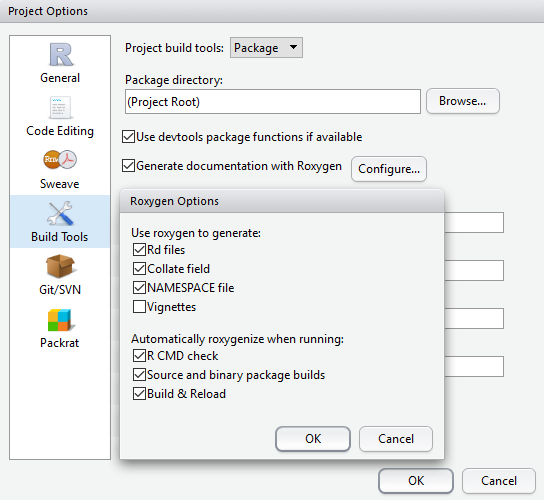
\includegraphics[width=0.7\textwidth]{abbildungen/build_config}
	\caption{Build- und Roxygen-Optionen des Projekts}
	\label{abb:build_roxygen_options}
\end{figure}
Nach der Implementierung der R-Skripte kann das endgültige R-Paket generiert werden. Dazu muss auf den \emph{Build \& Reload}-Button im \emph{Build}-Tab geklickt werden. Bei der Verwendung von C++-Code werden nun C++-Dateien kompiliert und R-Wrapper-Funktionen erstellt, die den Zugriff auf die C++-Funktionen erleichtern.
\\
\\
Eine C++-Datei muss mit folgenden Zeilen starten:
\begin{lstlisting}[language=C++, numbers=none, basicstyle=\ttfamily]
#include <Rcpp.h>
using namespace Rcpp;
\end{lstlisting}
Darüber hinaus muss jede Funktion, die in R verfügbar sein soll, folgenden Präfix erhalten:
\begin{lstlisting}[language=C++, numbers=none, basicstyle=\ttfamily]
// [[Rcpp::export]]
\end{lstlisting}
Am Ende des Build-Prozesses wird das Paket lokal installiert und ist bereit verwendet zu werden. Um das Paket auf anderen Rechnern installieren zu können muss im \emph{Build}-Tab via \emph{More~$\rightarrow$~Build Binary Package} das Paket zu einem Archiv gepackt werden. Dieses Archiv ist jedoch nur für Rechner mit demselben Betriebssystem geeignet, d.h. das Paket muss für jedes Betriebssystem separat kompiliert und gepackt werden.

\section{Faltungskodierer}
\label{kapitel:implementierung_faltungskodierer}
Ein Faltungskodierer ist gegeben durch 
\begin{itemize}
\item $N$: Anzahl an Ausgangsbits je Eingangsbit,
\item $M$: Länge des Schieberegisters,
\item $G$: Vektor von Generatorpolynomen.
\end{itemize}
Die Angabe von $M$ ist hier redundant, jedoch Teil der Benutzereingabe zur Generierung eines Faltungskodierers, welche durch \cite{morelos2006art} inspiriert wurde.
\\
\\
Zur leichteren Implementierung der Kodierung und Dekodierung wird die Kodierer-Datenstruktur um folgende Elemente erweitert:
\begin{itemize}
\item eine \emph{Zustandsübergangsmatrix}, die angibt, in welchen Zustand der Kodierer bei einem Eingangsbit wechselt,
\item eine \emph{inverse Zustandsübergangsmatrix}, die angibt, aus welchem Zustand der Kodierer bei einem Eingangsbit kommt,
\item eine \emph{Ausgabematrix}, die angibt, welche Kodebits der Kodierer bei einem Eingangsbit in einem bestimmten Zustand ausgibt,
\item ein Flag zur Markierung rekursiv systematischer Kodierer (RSC, siehe Kapitel~\ref{kapitel:grundlagen_rsc}),
\item ein \emph{Terminierungsvektor} der für rekursiv systematische Kodierer angibt, ob ein Eingangsbit 0 oder 1 in einem bestimmten Zustand für die Terminierung zu verwenden ist.
\end{itemize}
Die Implementierung der Matrizen wurde aus der Referenzimplementierung übernommen, musste jedoch erweitert werden, um für allgemeine Faltungskodes verwendbar zu sein. Für alle gilt, die Anzahl an Zeilen entspricht der Anzahl an Zuständen $2^{M}$. Der Zeilenindex entspricht dem Zustand. Die Zustandsübergangsmatrix sowie die Ausgabematrix besitzen jeweils zwei Spalten. Je eine Spalte steht für ein Eingangsbit (0 oder 1), wobei der Spaltenindex dem Eingangsbit entspricht. Die inverse Zustandsübergangsmatrix benötigt eine dritte Spalte. Für viele Kodierer (v.a. nicht-rekursive) tritt der Fall ein, dass nur durch ein bestimmtes Eingangsbit in einen bestimmten Zustand gewechselt werden kann. Sei ein Zustand bspw. nur durch das Eingangsbit 0 erreichbar, so bedeutet das, dass es für diesen Zustand mit dem Bit 0 zwei Vorgängerzustände gibt, für ein Eingangsbit 1 jedoch keinen Vorgänger. Diese zweite Möglichkeit wird in der dritten Spalte gespeichert. Nicht benötigte Felder der Matrix beinhalten den Wert -1. Alle Matrizen beinhalten dezimale Werte. Um die Bit-Werte zu erhalten, wie z.B. die Bits der Ausgabematrix, die für die Kodierung notwendig sind, muss mit bitweisen Shift-Operationen gearbeitet werden. Ein Codeausschnitt der Implementierung zur Erzeugung von Faltungskodierer ist in Listin~\ref{lst:generate_coder} zu sehen.
\\
\\
Der Terminierungsvektor ist für nichtrekursive Kodierer nicht notwendig, da ein Kode eines solchen Kodierers immer mit $M$ 0-Bits terminiert wird. Bei einem rekursiven Kodierer ist es nicht trivial zu sagen mit welchem Eingangsbit in einem bestimmten Zustand terminiert wird, um den Kodierer in den Nullzustand zu bringen. Dies hängt von der Definition des Rekursionpolynoms ab. Der Terminierungsvektor wird bei der Erzeugung rekursiver Kodierer berechnet.
\\
\\
Bei der Erzeugung von Faltungskodierern ist zu prüfen ob es sich um einen katastrophalen Kodierer handelt. RSC-Kodierer sind, wie in Kapitel \ref{kapitel:grundlagen_systematische_kodierer} beschrieben, nicht zu prüfen. Zur Prüfung wird nach dem Theorem von Massey-Sain (siehe Kapitel~\ref{kapitel:grundlagen_katastrophale_kodierer}) der größte gemeinsame Teiler der Generatorpolynome berechnet. Die Berechnung des größten gemeinsamen Teilers wurde mithilfe des euklidschen Algorithmus implementiert. Sowohl der euklidsche Algorithmus als auch die dafür notwendige binäre Polynomdivision wird an eine C++-Funktion delegiert.
\begin{lstlisting}[language=C++,caption=Codeausschnitt aus der Implementierung der C++-Funktion zur Erzeugung von Faltungskodierer, label={lst:generate_coder}, float=!th, basicstyle=\ttfamily\scriptsize]
for (int state = 0; state < NUM_STATES; state++) {
  for (int input = 0; input < 2; input++) {
    int current_state = (input << M) | state;

    int out = 0;
    for (int i = 0; i < N; i++) {
      int temp = sumDigits(current_state & generator[i], 2) % 2;
      out = (out << 1) | temp;
    }
    output(state, input) = out;
    nextState(state, input) = current_state >> 1;
  }
}

for (int state = 0; state < NUM_STATES; state++) {
  for (int input = 0; input < 2; input++) {
    if (previousState(nextState(state, input), input) == -1) {
      previousState(nextState(state, input), input) = state;
    }
    else {
      previousState(nextState(state, input), 2) = state;
    }
  }
}
\end{lstlisting}

\section{Kodierung}
\label{kapitel:implementierung_kodierung}
Bei Faltungskodes stellt die Kodierung den bei Weitem einfacheren Teil dar. Es muss lediglich jedes Bit der zu kodierenden Nachricht zusammen mit dem aktuellen Zustand, der nach jedem Bit mithilfe der Zustandsübergangsmatrix aktualisiert wird, auf die Ausgabematrix angewendet werden. Die Terminierung funktioniert analog, einzig das zu kodierende Bit muss ermittelt werden. Für RSC-Kodierer muss im Terminierungsvektor nachgeschaut werden, andernfalls ist das Terminierungsbit immer 0. Abgeschlossen wird die Kodierung mit dem Abbilden der Kodebits 0 bzw. 1 auf die Signalwerte +1 bzw. -1 nach Gleichung~\eqref{eq:bit_zu_signal_abbildung}. Algorithmus~\ref{algorithmus:kodierung} zeigt den Kodierungsalgorithmus.
\begin{algorithm}[H]
\renewcommand{\algorithmicforall}{\textbf{for each}}
\caption{Pseudocode der Faltungskodierung}
\label{algorithmus:kodierung}
\begin{algorithmic}[1]
\STATE state $=0$, code $=$ result $=$ " "
\FORALL {bit \textbf{in} message}
   \STATE output $=$ output.matrix[state][bit]
	\STATE code $=\mathit{concat}($code, output$)$
	\STATE state $=$ state.transition.matrix$[$state$][$bit$]$
\ENDFOR
\IF{terminate code}
   \FOR {$i=0$ \TO $M-1$}
      \STATE termination.bit $=$ rsc-coder $?$ termination.vector$[$state$]$ : $0$
      \STATE output $=$ output.matrix$[$state$][$termination.bit$]$
	   \STATE code $=\mathit{concat}($code, output$)$
	   \STATE state $=$ state.transition.matrix$[$state$][$termination.bit$]$
   \ENDFOR
\ENDIF
\FORALL {bit \textbf{in} code}
   \STATE signal $=1-2$bit
   \STATE result $=\mathit{concat}($result, signal$)$
\ENDFOR
\RETURN result
\end{algorithmic}
\end{algorithm}

\section{Dekodierung}
\label{kapitel:implementierung_dekodierung}
Die Dekodierung stellt bei Faltungskodes den wesentlich komplexeren Teil dar. Der Pseudocode des Viterbi-Algorithmus ist in Algorithmus~\ref{algorithmus:dekodierung} zu sehen. Der Algorithmus zeigt die hard decision Dekodierung, deren Implementierung im Folgenden diskutiert wird. Zunächst werden zu jedem Zeitpunkt die Metriken aller Zustände berechnet und in eine Matrix \texttt{metric} geschrieben. Die Metriken zum Zeitpunkt 0 werden initialisiert. Der Nullzustand, der dem Startzustand entspricht, wird mit dem Wert 0 initialisiert. Die restlichen Zustände zum Zeitpunkt 0 werden mit einer sehr hohen Metrik initialisiert, da es unmöglich ist, dass ein korrekter Pfad aus einem anderen Zustand als dem Nullzustand startet. Dadurch werden Pfade, die in diesen Zuständen beginnen, durch ihre hohe Metrik immer verworfen. 
\\
\\
Die verschachtelte Schleife in den Zeilen 3 - 14 implementiert den in Kapitel~\ref{kapitel:grundlagen_hard_decision} beschriebenen Algorithmus. Die \texttt{survivor.bit}-Matrix speichert (für jeden Zustand zu jedem Zeitpunkt) jenes der beiden Bits mit dem der Pfad mit der niedrigeren Metrik in den Zustand gelangt, d.h. nicht das letzte Bit des verworfenen Pfads, sondern das (letze) Bit des Pfads mit der niedrigeren Hamming-Distanz.
\\
\\
Im Anschluss werden die \emph{survivor states} gesucht. Diese entsprechen den Zuständen, die bei der Kodierung im Trellis durchlaufen werden. Aus ihnen kann, zusammen mit der \texttt{survivor.bit}-Matrix, die dekodierte Nachricht berechnet werden. Die Suche entspricht dem Backtracking. Zunächst wird der survivor state am Ende des Trellis gesucht. Wurde die Nachricht bei der Kodierung terminiert entspricht der survivor state dem Nullzustand. Andernfalls muss der Zustand mit der niedrigsten Metrik gesucht werden. Dieser wird dann zum survivor state. Die darauf folgende Schleife führt das Backtracking bis zum Zeitpunkt 0 fort.
\\
Im letzten Schritt wird die dekodierte Nachricht rekonstruiert.

\begin{algorithm}[H]
\renewcommand{\algorithmicforall}{\textbf{for each}}
\caption{Pseudocode der hard decision Dekodierung}
\label{algorithmus:dekodierung}
\begin{algorithmic}[1]
\STATE NUM.STATES $=2^{M}$
\STATE msg.length $=\frac{\mathit{length}(\mathrm{code})}{N}$
\FOR {$t=1$ \TO msg.length}
   \FOR {$s=0$ \TO NUM.STATES$-1$}
   	\STATE $m_{1}=$ metric$[t-1][\mathrm{prev.state}_1] + d_{H, \mathrm{prev.state}_1\rightarrow \mathrm{s}}$
   	\STATE $m_{2}=$ metric$[t-1][\mathrm{prev.state}_2] + d_{H, \mathrm{prev.state}_2\rightarrow \mathrm{s}}$
      \STATE metric$[t][s]=\mathit{min}(m_{1},m_{2})$
      \IF {$m_{1}<m_{2}$}
      	\STATE survivor.bit $=\mathit{bit}(\mathrm{prev.state}_1\rightarrow\ s)$
      \ELSE
      	\STATE survivor.bit $=\mathit{bit}(\mathrm{prev.state}_2\rightarrow\ s)$
      \ENDIF
	\ENDFOR
\ENDFOR

\IF{is.terminated}  
	\STATE survivor $=0$
\ELSE
	\STATE minimum $=$ metric$[$msg.length$][0]$
	\FOR {$s=1$ \TO NUM.STATES}
		\IF{metric$[$msg.length$][0]<$ minimum}
			\STATE minimum $=$ metric$[$msg.length$][s]$
			\STATE survivor $=s$
		\ENDIF
	\ENDFOR
\ENDIF
\STATE survivor.state$[\mathrm{msg.length}]=$survivor
\FOR {$t=\mathrm{msg.length}-1$ \TO $0$}
	\STATE $S=$survivor.state$[t+1]$
	\STATE survivor.state$[t]=$ previous.matrix$[S$, survivor.bit$[t+1][S]]$
\ENDFOR
\FOR {$t=1$ \TO msg.length}
	\STATE result $=\mathit{concat}($result, survivor.bit$[t][$survivor.state$[t]])$
\ENDFOR
\RETURN result
\end{algorithmic}
\end{algorithm}

\section{Rauschen}
\label{kapitel:implementierung_noise}
Um auch zeigen zu können, dass die Dekodierung auch tatsächlich für verrauschte Signale funktioniert, benötigt es eine Funktion, die die Übertragung einer Nachricht über einen verrauschten Kanal simuliert, d.h. das Signal mit Rauschen überlagert. Zum Signal soll ein additives weißes gaußsches Rauschen (AWGR oder AWGN\footnote{Additive White Gaussian Noise}) addiert werden um dieses zu verfälschen. In \cite{AWGN} wird eine alternative Implementierung zur eingebauten AWGN-Funktion in Matlab vorgestellt. Die Implementierung wurde übernommen bzw. nach R übersetzt. Durch die Möglichkeit das Signal-Rausch-Verhältnis über einen Parameter zu steuern, können verschiedene Übertragungskanäle simuliert und Nachrichten somit verschieden stark verrauscht werden. Der Benutzer kann dadurch herausfinden, ab wann eine Nachricht zu viel Rauschen enthält, um sie korrekt dekodieren zu können.

\section{Punktierung}
\label{kapitel:implementierung_punktierung}
Bevor ein Kode punktiert werden kann (siehe Kapitel~\ref{kapitel:grundlagen_punktierung}) benötigt es eine Punktierungsmatrix. Die Funktion zur Generierung einer Punktierungsmatrix bringt den vom Benutzer mitgegebenen Punktierungsvektor in die korrekte Matrixform.
\\
Zunächst wird der Punktierungsvektor überprüft, da dessen Länge ein Vielfaches von $N$ (Anzahl der Ausgänge des Faltungskodierers) sein muss. Nach der Transformation des Vektors zur Punktierungsmatrix wird geprüft, ob die Matrix eine Nullspalte enthält, da eine Nullspalte zur Folge hat, dass die 0-Werte vor der Dekodierung nicht eindeutig eingefügt werden können.
\\
\\
Für die Punktierung eines Kodevektors ist die Verwendung von Indexvektoren in R hervorragend geeignet. Die Punktierungsmatrix muss lediglich in einen logischen Vektor umgewandelt und als Indexvektor zwischen eckige Klammern hinter den Kodevektor geschrieben werden. Somit lässt sich die Punktierung, die mindestens gleich lang wie die Punktierungsmatrix sind, in nur einer R-Codezeile implementieren. Für kürzere Kodes muss einzig vor der Punktierung die Punktierungsmatrix auf die Kodelänge abgeschnitten werden.
\\
\\
Im Gegensatz zur Punktierung ist das Einfügen der 0-Werte mit mehr Aufwand verbunden. Vor allem die Berechnung der Anzahl an 0-Werten, die eingefügt werden müssen, ist für allgemeine Punktierungsmatrizen nicht trivial und wurde daher in eine C++-Funktion ausgelagert.\\
Die Anzahl an 0-Werten, die eingefügt werden müssen, berechnet sich für eine allgemeine Punktierungsmatrix $P \in {\left\lbrace 0,1 \right\rbrace}^{N\times \frac{p}{N}}$, die $q$ 1-Bits enthält, und ein punktiertes Kodewort $\mathbf{v}=\left( v_{1},v_{2},\dots ,v_{n}\right)$ wie folgt:
\begin{equation}
\mathit{zeros} = \left\lfloor \frac{n}{q} \right\rfloor \left(p-q\right)+m
\label{eq:punktierung_zeros}
\end{equation}
wobei $m$ der Anzahl an 0-Bits entspricht, die in den ersten $k$ Spalten der Punktierungsmatrix stehen, wobei $k$ dem kleinsten Wert entspricht, sodass die ersten $k$ Spalten mindesten $\left( n\mod q\right)$ 1-Bits enthalten. Für $n\mod q=0$ ist $m=0$.
\\
Der erste Summand ergibt sich aus der Anzahl, wie oft der punktierte Kode vollständig die 1-Bits der Punktierungsmatrix füllt, multipliziert mit der Anzahl an 0-Bits $\left( p-q\right)$. Die Anzahl an zusätzlichen 0-Werten $m$, die eingefügt werden müssen, ergibt sich aus den restlichen Kodebits, die die 1-Bits der Punktierungsmatrix nicht genau voll machen und dadurch vom ersten Summanden nicht berücksichtig werden.
\\
\\
Das Einfügen der 0-Werte ist einfach mithilfe einer Schleife, die die Punktierungsmatrix in jeder Iteration an der entsprechenden Stelle prüft und das depunktierte Kodewort aufbaut, zu implementieren.
\begin{beispiel}
Gegeben seien die punktieren Kodes \mbox{$\mathbf{v_{p,1}}=(110010)$} bzw. \mbox{$\mathbf{v_{p,2}}=(10011101001)$} mit einer Länge von 6 bzw. 11 Bits, sowie die Punktierungsmatrix
\begin{equation*}
P=
\begin{pmatrix}
1 & 0 & 1 \\
1 & 1 & 0 \\
\end{pmatrix}.
\end{equation*}
Nach Gleichung~\eqref{eq:punktierung_zeros} ergeben sich für $\mathbf{v_{p,1}}\ \left\lfloor \frac{6}{4} \right\rfloor \left(6-4\right)+0=2$ bzw. für $\mathbf{v_{p,2}}\ \left\lfloor \frac{11}{4} \right\rfloor \left(6-4\right)+1=5$ 0-Werte, die einzufügen sind. $\mathbf{v_{p,1}}$ füllt die 1-Bits der Punktierungsmatrix einmal vollständig, wodurch sich zwei zusätzliche 0-Werte ergeben. Die übrigen zwei Bits füllen die 1-Bits der ersten Spalte, welche keine 0-Bits enthält, daher kommen keine weiteren 0-Werte dazu. $\mathbf{v_{p,2}}$ füllt die die 1-Bits der Punktierungsmatrix zweimal vollständig, wodurch sich vier zusätzliche 0-Werte ergeben. Die übrigen drei Bits füllen die 1-Bits der ersten beiden Spalten, welche ein 0-Bit enthalten, daher kommt ein weiterer 0-Wert hinzu. Die depunktierten Kodes lauten \mbox{$\mathbf{v_{1}}=(11\mathbf{0}00\mathbf{0}10)$} bzw. \mbox{$\mathbf{v_{2}}=(10\mathbf{0}01\mathbf{0}11\mathbf{0}01\mathbf{0}00\mathbf{0}1)$}
\end{beispiel}

\section{Simulation}
\label{kapitel:implementierung_simulation}
Die Simulation führt ein Kodierungsverfahren für zufällige Nachrichten mehrmals für verschiedene Signal-Rausch-Verhältnisse durch. Dabei werden die Nachrichten kodiert, verfälscht und wieder dekodiert sowie die resultierende Bitfehlerrate (BER\footnote{bit error rate}), d.h. der Prozentsatz unterschiedlicher Bits zwischen originaler und dekodierter Nachricht, berechnet. Dieser Vorgang wird je Signal-Rausch-Verhältnis mehrmals durchgeführt. Die Bitfehlerrate ergibt sich aus dem Mittelwert aller Wiederholungen. Dadurch werden statistische Ausreißer vermieden. Bei der Dekodierung wird die soft decision Dekodierung verwendet.
\\
\\
Die Simulation kann über folgende Parameter gesteuert werden:
\begin{itemize}
\item Faltungskodierer, der für die Kodierung verwendet wird
\item Nachrichtenlänge der zufällig erzeugten Nachrichten
\item Sigal-Rausch-Verhältnisse, die getestet werden, durch Angabe von Minimum, Maximum und Schrittweite
\item Anzahl der Wiederholungen je Signal-Rausch-Verhältnis
\item Punktierungsmatrix (optional). Eine Punktierung erfolgt nur, falls eine Punktierungsmatrix mitgegeben wird.
\end{itemize}
Als Resultat wird ein Dataframe zurückgegeben, welches die Bitfehlerrate je Signal-Rausch-Verhältnis beinhaltet. Algorithmus~\ref{algorithmus:simulation} zeigt den Pseudocode der Simulation ohne Punktierung.
\begin{algorithm}[H]
\renewcommand{\algorithmicforall}{\textbf{for each}}
\caption{Pseudocode der Simulation}
\label{algorithmus:simulation}
\begin{algorithmic}[1]
\STATE total.errors $=0$
\STATE dataframe $=\emptyset$
\FOR {snr $=$ snr.min \TO snr.max \textbf{step} snr.interval}
	\FOR {$i=1$ \TO iterations.per.snr}
		\STATE msg $={\left\lbrace 0, 1\right\rbrace }^{\mathit{msg.length}}$
		\STATE encoded $=\mathit{encode}($msg$)$
		\STATE noisy $=\mathit{addNoise}($encoded$)$
		\STATE decoded $=\mathit{decode}($noisy$)$
		\STATE total.errors $+=\mathit{sum}($msg $\oplus$ decoded$)$
	\ENDFOR
	\STATE ber $=\frac{\mathrm{total.errors}}{\mathrm{msg.length}\ast\mathrm{iterations.per.snr}}$
	\STATE dataframe.$\mathit{add}($snr, ber$)$
\ENDFOR
\RETURN dataframe
\end{algorithmic}
\end{algorithm}
Neben der Simulation von Faltungskodes wurde eine Kanalkodierungs-Simulation implementiert. Diese führt die Simulationen aller Verfahren der Kanalkodierung, die im R-Paket implementiert worden sind  (Blockkodes, Faltungskodes und Turbo-Kodes), mit den gleichen Parametern aus und fasst die resultierenden Dataframes zusammen. Dadurch können die Verfahren mithilfe einer einzigen Funktion leicht miteinander verglichen werden.
%
\section{Visualisierung}
\label{kapitel:implementierung_visualisierung}
Die Visualisierung der Kodierung, Dekodierung und Simulation wurde mithilfe von \texttt{RMarkdown} (siehe Kapitel~\ref{kapitel:rmarkdown}) implementiert. Die Generierung der Beamer-Dokumente wird mithilfe des Befehls in Listing~\ref{lst:render_rmd} gestartet. Der erste Parameter entspricht der auszuführenden \texttt{RMarkdown}-Datei, inklusive Pfadangabe. Der \texttt{params}-Parameter kann verwendet werden, um der \texttt{RMarkdown}-Datei eine Liste von Parametern zu übergeben.
\begin{lstlisting}[caption=Erzeugen des Visualisierungs-Dokuments aus der RMD-Datei, label={lst:render_rmd}, float=!th]
rmarkdown::render("path/to/file/rmarkdown.rmd", params)
\end{lstlisting}
Listing~\ref{lst:open_rmd} zeigt die Funktion zum Öffnen des erstellten PDF-Dokuments.
\begin{lstlisting}[caption=Öffnen des Visualisierungs-Dokuments, label={lst:open_rmd}, float=!th]
rstudioapi::viewer("path/to/file/rmarkdown.pdf")
\end{lstlisting}

\begin{lstlisting}[caption=RMarkdown Header, label={lst:rmd_header}, float=!th]
title: "Faltungskodierung ohne Punktierung"
date: "`r format(Sys.time(), '%d %B, %Y')`"
output:
  beamer_presentation:
    keep_tex: true
params:
  message: !r c(1,0,1,1,0)
header-includes:
- \usepackage{tikz}
- \usepackage{pgfplots}
- \usepackage{mathtools}
- \usetikzlibrary{arrows,positioning,calc}
\end{lstlisting}
Listing~\ref{lst:rmd_header} zeigt einen Ausschnitt einer \texttt{RMarkdown}-Datei, wo der Header zu sehen ist. Zunächst werden Daten angegeben, die auf der späteren Titelfolie zu sehen sind, wie z.B. Titel und Datum. Im Anschluss werden die gewünschten Ausgabeformate definiert, wobei hier mit dem Beamer-Format nur eine Ausgabedatei erzeugt wird. Zusätzlich wird durch Zeile~5 die \TeX -Datei, die von \texttt{pandoc} zur Erzeugung des endgültigen Dokuments verwendet wird, abgespeichert. Schließlich werden die Parameter samt Standardwerten definiert, sowie Header inkludiert, die für die Ausführung des \LaTeX -Codes notwendig sind.
\\
Unterhalb des Headers folgt der Markdown-, R- und \LaTeX -Code der weiteren Folien. \cite{rmarkdown}